\documentclass[a4paper]{article}

%% Language and font encodings
\usepackage[english]{babel}
\usepackage[utf8x]{inputenc}
\usepackage[T1]{fontenc}
\usepackage{authblk}
\usepackage[usenames, dvipsnames]{color}
\usepackage[table]{xcolor}
%% Sets page size and margins
\usepackage[a4paper,top=2cm,bottom=2.4cm,left = 2 cm, right =2cm]{geometry}

%% Useful packages
\usepackage{amsmath}
\usepackage{amssymb}
\usepackage{graphicx}
\usepackage[colorinlistoftodos]{todonotes}
\usepackage[colorlinks=true, allcolors=blue]{hyperref}

\renewcommand*\familydefault{\sfdefault}
\usepackage[scaled = 0.92]{helvet}
\usepackage{hyperref}

%% define
\definecolor{odd_row}{RGB}{250,250,250}
\definecolor{even_row}{RGB}{217,217,217 }
\definecolor{header}{RGB}{197,197,197 }
\definecolor{footer}{RGB}{57,57,57 }
\font\titlefont=cmr9 at 30pt

%% define header and footer
\usepackage{fancyhdr}
\pagestyle{fancy}
\renewcommand{\headrulewidth}{0.4pt}
\renewcommand{\footrulewidth}{0.4pt}
\lhead{qplum Investment Research}
\rhead{
\includegraphics[width=2cm]{qplum_logo.png}}
\cfoot{\color{footer}\footnotesize
\normalsize\thepage
}


\author[1]{Puru Sarathy \thanks{puru.sarthy@circulumvite.com}}
\author[1]{Ankit Awasthi\thanks{ankit.awasthi@circulumvite.com}}
\author[1]{Diwakar Chauhan\thanks{diwakar@circulumvite.com}}
\author[1]{Hrishav Agarwal\thanks{hrishav@tworoads.co.in}}

\affil[1]{qplum Investment Research}

\title{Walk-forward Approach to High Frequency Trading}
\date{}


\begin{document}

\maketitle

\begin{abstract}
The term Walk-forward refers to a protocol of testing ideas in a time series context by strictly adhering to a no-lookahead bias policy while creating and testing one's ideas. Walk-forward strategies in a high frequency domain refer to approaches to generate a trading idea for the next day given all or some of the data we have seen till date. We explore various formulations of this broad concept and show some examples as applied to high frequency trading.
\end{abstract}


\section{Motivation}

Traders have often observed that re-tuning their strategies to recent data often is useful in obtaining better strategies. One obvious case for a trader in high frequency trading is that her product standard-deviation has changed recently and she would like to adapt in a dynamic fashion to this change. The other case would be when her product has started following a different source product. A possible ill-effect of this is that strategies to trade a product become over-fitted to look-ahead data and there is no way to prevent this as traders go about their process of refining their strategies. Recent parameter setting for entry-exit of trades also do better than older parameter settings and is another area prone to look-ahead bias and over-fitting. All of these observation lead us to think about a walk-forward setup where we have configurations (hereby known as configs) to produce different effects in trading. We will elaborate further on these configurations for walk-forward in the next section.

\section{Overview of automated trading strategy development\label{overview}}
An intra-day focused trading strategy is typically based on a ``model'' of markets and a set of parameters ``paramset'', that we use to take trading decisions. An old-school approach to finding good trading strategies was to take a bunch of data and find the model and paramset that would have had the highest profits on that data. Let's look at a few improvements quantitative portfolio managers employed in an effort to reduce over-fitting to past data and to improve trading profits in future unseen data.\\
An improvement in the optimization step of searching for strategies was to change the search criterion from highest profits to a a more stable measure of profits like Sharpe Ratio. The motivation was that we are looking for strategies that have a stable income stream and not just one that would have made an occasional windfall. Strategies with sporadic sources of returns might go long patches in future without returns.\\
Another improvement made by the quantitative community was to split the data into training data and testing data every time the model was retrained. The portfolio manager, a.k.a PM, would make sure to only choose models whose performance does not degrade substantially between training and testing period. However, it was often very difficult to employ this method in finance. There are frequent regime shifts, correlations between different products change all the time. Market volatility can change, it can suddenly become much more volatile than it used to be earlier. There is a large body of research that shows heteroskedasticity in markets and that volatility in markets goes up fast and comes down slowly. A PM trying to find a strategy to trade with tomorrow will probably think today's and yesterday's data to be relevant. They would not care about data a year back for instance. Now if we include today's data in training then we cannot include it in testing period. Then even if the results deteriorate in testing then the PM might feel that the deterioration is to be expected and training on most recent data has allowed them to capture the seasonality in finance. This is why the traditional method of splitting data between training and testing does not work in finance.
Even with all the work above there is established evidence of degradation of results between backtest and real trading performance [reference here]. We believe that there is nothing fundamentally wrong in a portfolio manager using recently available data in retraining their models. Only improvement they can make is to find data in the past that is behaviorally very similar to recent data. However, the major source of degradation of results is the way we measure expected performance.\\

%% \cite{Suhonen2016}

In real life, the portfolio manager would be making changes periodically based on new data. For instance, if the market has become very volatile and we see that our paramset is not well adjusted to this new regime, the portfolio manager would want to recalibrate the paramset to this new regime, since it typically continues for a while. In this process of retraining, as it happens most of the time, the PM will end up choosing a paramset that makes the backtested results look good. These backtested results would be too optimistic a prediction of what we are likely to see in real trading if we trade with the newly retrained strategy.\\
The right way to measure expected profits would require us to see this strategy updation process as an essential part of the pipeline and to ensure that we never measure expected profits on a trading day with a strategy that would have been constructed looking at data not available till the day before.

The problem we are trying to solve in this paper is how to build a system where the PM is allowed access to the most recent data when they retrain their strategy and yet we measure the new strategy on strictly out of sample data that is likely to be very relevant to the trading day the strategy was retrained for. The solution we propose is a strict adherence to Walk-Forward optimization.

\subsection{Walk-forward strategy updation pipeline}
Walk-forward strategy updation pipeline refers to the set of steps that decide what model and paramset to use the next day. In other words, instead of populating our pool of eligible options to trade today with strategies and updating them every so often, we need to create a pool of strategy pipelines or "walk-forward configs". This would ensure that when it comes to choosing among the available options we have a way of measuring their performance on truly "out of sample" data. So instead of strategies we will have only configs in the pool for the product. At any point the trader only chooses the config, i.e. what methodology should she use to decide the model and paramset for tomorrow? The advantage here being that we have an accurate measure of the performance of this methodology in the historical results.

\subsection{How to transition to walk-forward configs in a non-disruptive fashion}
An engineering approach to transitioning to walk-forward configs would be directly tackle the problem of making the best walk-forward config. However, in practice we have seen that this might not be the best approach. That is a very tough problem and for a company looking to transition from the traditional strategy construction workflow to a walk-forward config based workflow, this might be a very long process. Our advice is to implement a walk-forward config based on a strategy updation logic you already believe in, and think is appropriate for the product at hand.\\
Some people believe in updating a linear regression model every month and calibrating the paramset every day. They should implement the same as a walk-forward strategy where we are doing this everyday and simulating the performance of this strategy on the next day's data. Let's call this Type 1.\\
Some people would not care about RSquared and would want to choose based on what maximizes the Sharpe Ratio of PNL. They should do the same. Let's call this Type 2.\\
Some people believe in not updating the model and paramset at all. Even this can be written as a special case of a walk-forward strategy. Let's call this Type 3. However, in this case we will need to remember the last day that the model and paramset were updated and we need to make sure that we do not include backtested results of any day prior to the strategy creation date when we are figuring out the expected returns in future.\\
Some people believe in updating the paramset based on the current market trading volume or the current market volatility. Let's call it Type 5. They should try to create a walk-forward config that uses this approach.\\
As an organization, we should try not to waste time tackling the ``ML-hard'' problem of ``what is the best walk-forward config'' and use one's intuition about the product (or existing know-how from other traders) to come up with the right walk-forward type.

\subsection{Why this transition really needs a rethink}
One bad way of transitioning to walk-forward configs is the following. Suppose a company has a long history of working with old school strategies, and the portfolio managers have a lot of political clout to ignore over-fitting. They could, for instance, continue to make strategies the old way and make a new model and paramset every time they retrain and just convert it into a Type 3 config. The risk management division will need to be cognizant of the over-fitting risks of trading with a strategy that was just made and hence to deter the strategy from being selected by the strategy selector.\\
We need to think about writing pipelines and configs such that we don't have to change them for years. That might be an ambitious target, however that mindset is very important while writing the pipeline. The end goal of this exercise is to create a process by which we find pipelines that capture all the actions we would take as a portfolio manager overnight. We have consequently made sure that we are not overfitting any more and we only simulating a strategy on a trading day that is strictly later than every day of data used to make that trading strategy.

\section{Different walk-forward configs: Descriptions}
\subsection{Example 1: Type 4 Config}
The usual trading idea in high frequency domain is to combine a model and a parameter file. The model file controls the directional input to the strategy and the parameter file controls when to enter and exit the position. Further details on maximum position and other higher order book behavior is controlled by the parameter file. Often when near term volatility is higher, the parameter file needs to be readjusted to control for excess trading. This is done typically by a trader as a linear search in the entry-exit parameter, with the objective function being the near term backtest profit and loss numbers. One consequence of this protocol is potential over-fitting. It is hard to determine whether the readjusted parameter file is over-fitted to recent performance, in that whether or not it will serve business interests in the near out of sample future is not clear. We hope to solve these problems with the idea of a type 4 walk-forward config.

A type 4 configuration accepts a list of parameter files along with a model file. At any point in the trading of this configuration, a decision is made on which parameter file is to be used by looking at the performance of the model combined with all the given parameter files in the recent history before that date. Trader can specify the criteria for this search, i.e. how many days to look back and how to sort the results (Pnl and Sharpe Average/Drawdown based). Once the parameter file is chosen, the configuration is ready to trade the next day. In evaluating the performance of this configuration, the same procedure is followed strictly through the time series of dates to evaluate the profit and loss metrics as we walk-forward in time.

Another variant of a type 4 config is one that uses various models and a single param. A classic example here is CGB. We know that often the correlation of CGB with ZN and CL changes around frequently. If we were a smart PM making a decision on this, we would pick our models based on 
what the recent correlations with ZN, CL and BAXMID looks like. We present this study in the research section later in this document.

\subsubsection{Discussion: Type 4 Config}
Two immediate concerns about the type 4 config are
\begin{enumerate}
\item Computation complexity of generating results for all the sub-strategies
\item Possible overfitting in the result space with bad out of sample performance
\item Convergence to similar strategies
\end{enumerate}
The first problem cannot be simplified at the unit level (the time it takes to simulate one strategy for a day is fixed), however we can kick off parallel jobs to ease some of this burden. The second useful trick is around deciding how to group dates for running simulations. Imagine a type 4 config that needs to decide its model and parameter on each day in the past year, its pretty straightforward that we need results for each sub-strategy for each date. However, if one some days the model and parameter already exists, we can optimize the calls to the simulations process given the set of dates and the lookback period.

The second and third problems are more complex. Fitting strategies using backtest results would have this drawback, one can avoid this by being not too reactive (lookback days need to be larger than, say a given number of days). Convergence to similar strategies can be avoided by using different settings on each seed strategy, where seed strategy is a strategy that one can start with to build a configuration.

\subsection{Example 2: Type 5 Config}
A type 5 config is based on sample features. We define sample features to be a set of market structure related features on a product in a time period. Typically sample features are defined over fifteen minute time intervals, for example, the level one book size could be a sample feature, the average order size traded in the interval could be another. A type 5  config is one that uses history on sample features to pick different parameter files. A period is specified by the trader as a lookback, if the sample feature is below a cutoff, the first param file is used. Otherwise, the second one is used. Often we find that parameters of the trading change with L1 book size, this problem is directly handled by a type 5 config.

One easy starting point for a type 5 config is to think about what sample features affect trading in the product. For example, we know that for Hong Kong the standard deviation of the product largely determines what kind of trading we do. To use this observation in a walkforward setting, we can train models separately on high standard deviation days and low standard deviation days and switch between these two models based on last five day standard deviation.






































\begin{centering}
	\begin{figure}
		
		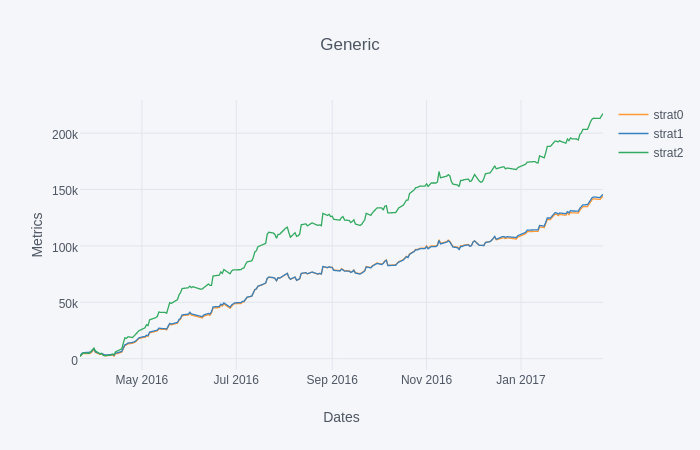
\includegraphics[scale=0.7]{type5.png}
		
		\caption{An improvement with a type5 config - this config was such that it took more intra day positions when book sizes are larger.}
		\label{fig:type5}
		
	\end{figure}
\end{centering}

Figure \ref{fig:type5} shows an example of a type 5 config applied to a product.




\section{Research Results on Walkforward ideas}
\subsection{Exploring different models and sort-algos}
One study exploring different models was done on various products and sessions. The setup is the following. For each product session there is a list of models, and existing param, and a set of sort algos. The goal was to see if we can decide which sort algo is the best choice. The results on all possible strategies are computed and results are sorted using the five sort algos. Corresponding to each sort algo, there is a strategy, and we run that to generate five out of sample profiles. Which sort algo wins? 

In more detail, we choose a few EUREX products for US session(FGBM, FGBL, FDAX, FESX). These products were chosen as their pool had old strats(thereby, providing a fair comparison against walkforward configs). Their volatility had varied a lot last year, so they were possibly a good case for the experiments. For each products, we chose strats with paramfiles that are common in the pool, but are varied amongst themselves in thresholds. The dates for selection of strats and params: 2015/10 - 2015/12 and dates for evaluation of configs: 2016/01 - 2017/01 (a period of one year). Candiate lookback days are 5,12 and sort-algos were Sharpe, PnlAvg, Pnl/DrawDown (PnlDD).

Results link:
%\href{https://docs.google.com/spreadsheets/d/1IvCSVy-Fs4tgkKbMTND4JB6CK%l3i%DQgCxsP8ePn69NE/edit#gid=208791336}
 
%\href{www.google.com}


Summary: 
15day PnlDD was found to be best performing in most strategies.
Sharpe as metric does not do so well (particularly for short lookback days)
For all shortcodes, the config is doing better that strats for most cases.
One point here to be noted is that configs for different strats become very similar (owing to same paramlist taken for configs)



So Surprisingly the answer to this is the PNLBYDD algo, that almost always consistently outperforms. In other words, for the PM using PNLBYDD might be a smart way to sort possible strategies.


Another line of experimental design was around choosing from diverse models based on simulation PNL. We chose a vast range of products including XT, AP, ZN, FGBM, FOAT, TOPIX which have varying regimes (hence model-selection might be an asset).

Similar to that in param-space, we asked the individual traders to provide a list of strats with diverse models (diverse in terms of sources or indicators). We considered price based aggressive trading strats for this experiment. Dates for selection of strats and params was 2015/10 - 2015/12
and dates for evaluation of configs was 2016/01 - 2017/01.


Again we found that 15 Day PNLDD was a good metric. Most of these configs performed similar or slightly better than the strats. One point to note was the convergence effect to the same strategy was even more in this case, but that was expected because this is done in the PNL space.


Results link: 
%https://docs.google.com/spreadsheets/d/1VvZhtNwzJ9yzYm16tQ6TBA1VayroOeFxBHplusFWmNY/edit#gid=1308102465


\section{Problems faced in transitioning to Walk-Forward configs \label{problems}}
\subsection{Operational Difficulties}
	
	A lot of our trading relies upon an existing workflow. One good example is the generate strategies workflow. This involves a set of steps that minimizes the effort of the part of the trader. All she needs to do is come up with a list of indicators and params and the perl script takes care of everything. In walkforward there is yet to be such easy infrastructure to let's say create a type 5 config. It requires a lot more intermediate steps.
	
	
	Secondly, a lot of our strategy search's success depends upon effective randomization. For example, randomizing data filters and sampling parameters. This randomization helps the trader search for alpha over a large space, which is restricted by some broad boundaries. In walkforward this space is operationally less searchable as of this point, mostly because of lack of infra-structure on this front.
	
	\subsection{Idealogical Difficulties}
	Walkforward ideas are not that easy to generate. They require considerable experience on a product. For DVC being a company that has mixed experience profiles, jumping to walkforward configs for all products may be ambitious.  
	
	Walkforward ideas are less generalizable. For example, if i want to switch model based on something more complicated than a sample feature, we don't have any ready support to solve that problem yet.
	
	\bibliographystyle{alpha}
	\bibliography{refs}
	\newpage
	\section{Disclosures \label{disclosures} }
	All investments carry risk. This material is for informational purposes only. The factual information set forth herein has been obtained or derived from sources believed to be reliable but it is not necessarily all-inclusive and is not guaranteed as to its accuracy and is not to be regarded as a representation or warranty, express or implied, as to the information’s accuracy or completeness, nor should the attached information serve as the basis of any investment decision. Past performance is not indicative of future performance. Please visit our website \url{https://www.qplum.co/privacy-terms#disclaimer} for full disclaimer and terms of use.\\
	This document is intended exclusively for the use of the person to whom it has been delivered and it is not to be reproduced or redistributed to any other person.
	
\end{document}

